Dado un conjunto de rectángulos alineados con el eje, ¿cuál es el área de su unión? Al igual que el problema de la intersección de líneas, podemos manejar esto tratando con eventos y conjuntos activos. Cada rectángulo tiene dos eventos: borde izquierdo y borde derecho. Cuando cruzamos el borde izquierdo, el rectángulo se agrega al conjunto activo. Cuando cruzamos el borde derecho, se elimina del conjunto activo.

% TODO: \usepackage{graphicx} required
\begin{figure}[h!]
	\centering
	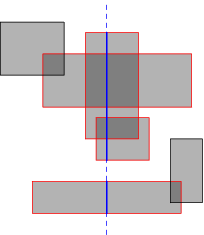
\includegraphics[width=0.2\linewidth]{img/rects}
	\label{fig:rects}
\end{figure}

Ahora sabemos qué rectángulos corta la línea de barrido (roja en el diagrama), pero en realidad queremos saber la longitud de la línea de barrido que se corta (la longitud total de los segmentos azules sólidos). Al multiplicar esta longitud por la distancia horizontal entre eventos, se obtiene el área barrida entre esos dos eventos.

Podemos determinar la longitud de corte ejecutando el mismo algoritmo en un bucle interno, pero girado 90 grados. Ignore los rectángulos inactivos y considere una línea de barrido horizontal que se mueve de arriba hacia abajo. Los eventos ahora son los bordes horizontales de los rectángulos activos, y cada vez que cruzamos uno, podemos simplemente incrementar o disminuir un contador que dice cuántos rectángulos se superponen en el punto actual. La longitud de corte aumenta siempre que el contador no sea cero. Por supuesto, no lo aumentamos continuamente, sino mientras pasamos de un evento a otro.

Con las estructuras de datos correctas, esto se puede implementar en tiempo O($N^2$) (sugerencia: use una matriz booleana para almacenar el conjunto activo en lugar de un árbol binario balanceado, y ordene previamente todo el conjunto de bordes horizontales). De hecho, el barrido de la línea interna se puede reemplazar con una manipulación inteligente del árbol binario para reducir el tiempo total a O ($N \log N$), pero eso es más un problema en las estructuras de datos que en la geometría, y se deja como un ejercicio para el lector. El algoritmo también se puede adaptar para responder preguntas similares, como la longitud total del perímetro de la unión o el número máximo de rectángulos que se superponen en cualquier punto.